% !TEX root = manuscript.tex

\chapter{Conceptual Framework}%\chapter{Key Features of \acs{3GPP} \acs{5G} Standards}%\chapter{\acs{5G} Scenario}%{System Modeling}
\label{chp:theory}

%\addbibresource{../resource/ref.bib}

This chapter is divided into two parts, in each one we give an overview of a subject, mainly:
\begin{enumerate}
    \item The first part will give an overview of the transmission of downlink data, as well as some of the \gls{phy} procedures associated with it.
    \item The second part will give an overview of some fundamental concepts of \gls{rl}.
\end{enumerate}

\section{Transmission Procedures}
\label{sec:5gnr-trans}
% Transport Channel Processing on 5G NR
\Gls{mac} uses services from the physical layer in the form of transport channels.
%
A transport channel defines how the information is transmitted over the radio interface \cite{3gpp.38.212} \cite{ErikDahlman5G}.
%
The transport channels defined for 5G-NR in the downlink are \gls{dlsch}, \gls{pch}, and \gls{bch}. In the uplink there are two transport channels, \gls{ulsch} and \gls{rach}.
% Downlink transmissions make use of  \gls{dlsch}, \gls{pch} and \gls{bch}. In the uplink, the transport channel is called \gls{ulsch}.
%
% The data transmissions in the downlink use the \gls{dlsch} and in the uplink the \gls{ulsch} \cite{AliZaidi632018}.
Downlink data uses the \gls{dlsch}, while the uplink uses the \gls{ulsch} \cite{AliZaidi632018}.
%

Each transport channel is mapped to some physical channel, with a physical channel corresponding to a set of time-frequency resources used for transmission.
%
This transmission can be of transport channel data, control information, or indicator information.
%
The physical channels without the corresponding transport channel are used for conveying the \gls{dci} and \gls{uci} \cite{ErikDahlman5G}.
%
The physical channels defined for \gls{5g} \gls{nr} are \cite{3gpp.38.211}:

\begin{enumerate}
    \item \Gls{pdsch}: used not only for downlink data transmission, but also for random-acess response messages, parts of the system information and paging information.
    %
    \item \Gls{pdcch}: used for \gls{dci}, that includes scheduling decisions needed for the reception of downlink data and scheduling grants for uplink data transmission.
    %
    \item \Gls{pbch}: used for broadcasting system information needed by the device to access the network.
    %
    \item \Gls{pusch}: used for uplink data transmission.
    %
    \item \Gls{pucch}: used for \gls{uci}, that includes \gls{harq} acknowledgments, scheduling request and downlink \gls{csi}.
    %
    \item \Gls{prach}: used for random access.
\end{enumerate}

The mapping of transport channels and control information to physical channels is depicted in Figure \ref{fig:channel-mapping}.

\begin{figure}[htbp]
    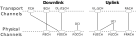
\includegraphics[width=0.95\columnwidth]{figures/chp_theory/complete.pdf}
    \caption{Mapping of transport channels to physical channels}
    \source{Created by the author based on \cite{ErikDahlman5G}}
    \label{fig:channel-mapping}
\end{figure}


Data in the transport channel is organized into transport blocks. For each component carrier and at each \gls{tti}, up to two \glspl{tb} are conveyed to the physical layer and transmitted over the radio interface  \cite{ErikDahlman5G}.
%
The transmission process is summarized in Figure \ref{fig:transmission}.
%
This process is similar for the uplink and downlink, the only difference being the additional step of transform precoding after the layer mapping in the uplink case.

\begin{figure}[htbp]
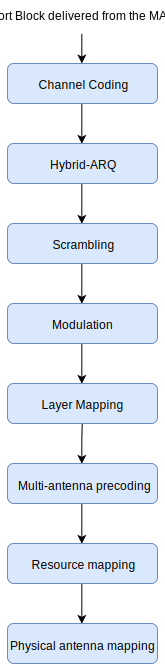
\includegraphics[width=\columnwidth]{figures/chp_theory/transmissionmodel.pdf}
\caption{General transmission model on \gls{5g} \gls{nr}}
\label{fig:transmission}
\end{figure}
%
In the modulation phase, \gls{nr} supports \gls{qpsk} and three orders of \gls{qam}, namely 16\gls{qam}, 64\gls{qam} and 256\gls{qam}, for both the uplink and downlink, with an additional option of $\pi/2$-BPSK in the uplink.
%
The \gls{fec} code for the \gls{embb} use case in data transmission is the \gls{ldpc} code, whereas in the control signaling polar codes are used.
%

In our work, we are mainly concerned with the \gls{pdsch} transmissions, in this case the overall \gls{5g} \gls{nr} channel coding process comprises six steps \cite{ErikDahlman5G}, namely:
\begin{itemize}
	\item \Gls{crc} Attachment: Calculates a \gls{crc} and attaches it to each transport block. It facilitates error detection and its size can be of 16 bits or 24 bits.
	\item Code-block segmentation: Segments the transport block in the case of it being larger in size than the supported by the \gls{ldpc} coder. Produces \gls{cb} are of equal size.
	\item Per-\gls{cb} \gls{crc} Attachment: A \gls{crc} is calculated and appended to each \gls{cb}.
	\item \gls{ldpc} Encoding: The solution used in \gls{nr} is a Quasi-cyclic \gls{ldpc} with two base graphs, the two base matrices that are used to built the different parity-check matrices with different payloads and rates.
	\item Rate Matching: It adjusts the coding to the allocated resources. It consists of bit selection and bit interleaving.
	\item Code-Block Concatenation: Concatenates the multiple rate-matching outputs into one block.
\end{itemize}

The other blocks in Figure \ref{fig:transmission}, excluding the channel coding and the modulation, are:
\begin{enumerate}
	\item \Gls{harq}: \gls{5g} \gls{nr} uses \gls{harq} with soft combining as the primary way to handle retransmissions. In this approach, a buffer is used to store the erroneous packet and this packet is combined with the retransmission to acquire a combined packet, which is more reliable than its components.
	%
	\item Scrambling: The process of scrambling is applied to the bits delivered by the \gls{harq}. Scrambling the bits makes them less prone to interference.
	%
	\item Layer mapping: The process of layer mapping is applied to the modulated symbols. It distributes the symbols across different transmission layers.
	%
	\item Multi-antenna precoding: This step uses a precoder matrix to map the transmission layers to a set of antenna ports.
	%
	\item Resource mapping: This process takes the symbols that should be transmitted by each antenna port and maps these to the set of available resource elements.
	%
	\item Physical antenna mapping: Maps each resource to a physical antenna.
\end{enumerate}

The \gls{pdsch} has only one defined transmission scheme \cite{3gpp.38.214}.
%
In this scheme the downlink transmission can be performed with up to 8 transmission layers on antenna ports 1000-1011.
%


In the following subsections we give an overview of the \gls{5g} \gls{nr} \gls{ldpc} coding solution and a more detailed explanation of some of the \gls{pdsch} procedures in Figure \ref{fig:transmission}.


%%%%%%%%%%%%%%%%%%%%%%%%%%%%%--subsection--%%%%%%%%%%%%%%%%%%%%%%%%%%%%%%%%%

\subsection{The \gls{5g} \gls{nr} \gls{ldpc}}

% %
% Before explaining the \gls{cb} segmentation and the \gls{ldpc} encoding, we will present some introduction to the coding solution applied to the \gls{embb} use case in the \gls{5g} \gls{nr}.
% %

\Gls{ldpc} codes are a class of linear block codes based on a sparse \gls{pcm}  originally proposed by Gallager \cite{gallager1962}.
%
Several standards have incorporated \gls{ldpc} codes, such as IEEE 802.11n, IEEE 802.16e (WiMAX) and \gls{dvb-s2} \cite{AliZaidi632018}.
%
In the third and forth generations (3G and 4G) turbo codes were the primary coding scheme \cite{Richardson2018} and were one of the candidates for the \gls{5g} \gls{nr} along with polar codes and \gls{ldpc} codes \cite{Hamidi8417496}.
%
The \gls{5g} \gls{nr} will make a transition on the error correcting codes with the \gls{ldpc} codes being used for the data channel and polar codes being used for the control information, on both the \gls{embb} and in the release-15 \gls{urllc} use cases \cite{bae_abotabl_lin_song_lee_2019}.

Although turbo codes and \gls{ldpc} codes have similar error-correcting capabilities \cite{ErikDahlman5G}, \gls{ldpc} codes provide the following advantages \cite{Hui2018}:

\begin{enumerate}
    \item Higher coding gains
    \item Lower error floors
    \item Higher achievable peak throughput
    \item Lower decoding complexity and improved decoding latency, particularly on high code rates
    \item Can achieve greater parallelism when decoding
\end{enumerate}

In a $(n, k)$ \gls{ldpc} code, the \gls{pcm} is a $ (n-k) \times n$ sparse matrix, with $k$ being the number of information bits and $n$ being the number of code-word bits, i.e information bits plus parity bits.
%
The sparseness of the \gls{pcm} enables a relatively simple decoding by making use of low-complexity iterative decoding algorithms.
%
The \gls{pcm} can also be represented by a graph connecting $n$ variable nodes with $(n-k)$ check nodes, the check nodes correspond to the parity-check equations.
%
In this graph there is an edge between a variable node and a check node if the corresponding entry on the \gls{pcm} is not-null \cite{Richardson2018}.
%
This bipartite graph representation is known as Tanner graph \cite{TannerGraph} and is the reason that the term \glsfirst{bg} is used in the \gls{nr} specifications.
%


The \gls{nr} \gls{ldpc} codes are \gls{qc} \gls{ldpc} codes, a class of photograph codes \cite{bae_abotabl_lin_song_lee_2019}.
%
In \gls{qc}-\gls{ldpc} the \gls{pcm} is constructed based on a smaller photograph, also called base matrix or \gls{bg}, that describes the macroscopic structure of the code \cite{Richardson2018}.
%
The \gls{pcm} can then be constructed by replacing each entry of the base matrix by a $\gls{not:lift-factor} \times \gls{not:lift-factor} $ cyclic permutation matrix, this process is called lifting and $\gls{not:lift-factor}$ is the lifting size.
%
In a Tanner graph representation, the lifting procedure is equivalent to having the larger graph being formed by $\gls{not:lift-factor}$ copies of the \gls{bg} and permuting the edges \cite{bae_abotabl_lin_song_lee_2019}.
%
One important consequence of this structure is that, with the higher possible parallelism, the decode complexity is a function of the \gls{bg} size, not of the actual \gls{pcm} size, since it can be achieved a degree of parallelism of $\gls{not:lift-factor}$ \cite{bae_abotabl_lin_song_lee_2019}.
% The \gls{nr} specifies the maximum $\gls{not:lift-factor}$ to $384$.

% TODO: Figure of tanner graph here


In the \gls{5g} \gls{nr} \gls{ldpc} code, each ``0'' in the \gls{bg} is replaced by a $\gls{not:lift-factor} \times \gls{not:lift-factor} $ all-zero matrix and each ``1'' is replaced by a circularly shifted identity matrix, shifted by the corresponding shifting coefficient \cite{ErikDahlman5G}.
%
In the technical specification \cite{3gpp.38.212}, 51 lifting sizes are specified and they are divided in 8 groups, called set index $\gls{not:set-index}$, each set index corresponds to a different permutation design, i.e different shifting coefficients, this structure is resumed in the Table \ref{tab:lift-table}.
%
This design means that there are 51 \glspl{pcm} for each of the two \glspl{bg}.

\begin{table}[htb]
\centering
\caption{Sets of \gls{ldpc} lifting sizes}
\label{tab:lift-table}
\begin{tabular}{l c}
  \toprule
  Set index $\gls{not:set-index}$   & Set of lifting sizes $\gls{not:lift-factor}$ \\
  \midrule
  0  &  2, 4, 8, 16, 32, 64, 128, 256 \\
  1  &  3, 6, 12, 24, 48, 96, 192, 384 \\
  2  &  5, 10, 20, 40, 80, 160, 320 \\
  3  &  7, 14, 28, 56, 112, 224 \\
  4  &  9, 18, 36, 72, 144, 288 \\
  5  &  11, 22, 44, 88, 176, 352 \\
  6  &  13, 26, 52, 104, 208 \\
  7  &  15, 30, 60, 120, 240 \\
  \bottomrule
\end{tabular}
\source{\cite[Table 5.3.2-1]{3gpp.38.212}}
\end{table}


Two \glspl{bg} are specified in \gls{5g} \gls{nr}, in order to guarantee efficiency for all the payload sizes and code rates.
%


%%%%%%%%%%%%%%%%%%%%%%%%%%%%%--subsection--%%%%%%%%%%%%%%%%%%%%%%%%%%%%%%%%%
\subsection{\Acl{mcs} and \acl{tbs} determination}

To start the decoding process the \gls{ue} must first determine the modulation order, the target code rate and the \glspl{tbs} in the \gls{pdsch}.
%
To determine this the \gls{ue} needs some information:

\begin{enumerate}
    \item The \gls{mcs} index, $I_{mcs}$, which is a 5-bit field in the \gls{dci}.
    %
    \item The redundancy version, which is used for the \gls{harq} functionality on the rate-matching step of the channel coding and is a 2-bit field included in the \gls{dci}.
    %
    \item The number of layers.
    \item The number of allocated \glspl{prb} before the rate matching.
\end{enumerate}

The \gls{mcs} index is used alongside a table to determine the modulation order and the target code rate.
%
Until the writing of this work only three \gls{mcs} tables were defined in the the technical specification \cite{3gpp.38.214}, two of modulation order up to 64\gls{qam}, with one of those used for a low spectral efficiency case, and one with modulation order going up to 256\gls{qam}.
%
In this work we used the table \cite[Table 5.1.3.1-2]{3gpp.38.214}, that goes up to 256\gls{qam}, reproduced in Table \ref{tab:mcs-table}, where \gls{not:rate} is the target code rate:

\begin{table}[htb]
\centering
\caption{\gls{mcs} index table 2 for \gls{pdsch}}
\label{tab:mcs-table}
\begin{tabularx}{0.95\columnwidth}{l X X r}
  \toprule
  \gls{mcs} index  & Modulation order & \gls{not:rate} x 1024  &  Spectral efficiency \\
  \midrule
  0  &  2   & 120       &  0.2344 \\
  1  &  2   & 193       &  0.3770 \\
  2  &  2   & 308       &  0.6016 \\
  3  &  2   & 449       &  0.8770 \\
  4  &  2   & 602       &  1.1758 \\
  5  &  4   & 378       &  1.4766 \\
  6  &  4   & 434       &  1.6953 \\
  7  &  4   & 490       &  1.9141 \\
  8  &  4   & 553       &  2.1602 \\
  9  &  4   & 616       &  2.4063 \\
  10 &  4   & 658       &  2.5703 \\
  11 &  6   & 466       &  2.7305 \\
  12 &  6   & 517       &  3.0293 \\
  13 &  6   & 567       &  3.3223 \\
  14 &  6   & 616       &  3.6094 \\
  15 &  6   & 666       &  3.9023 \\
  16 &  6   & 719       &  4.2129 \\
  17 &  6   & 772       &  4.5234 \\
  18 &  6   & 822       &  4.8164 \\
  19 &  6   & 873       &  5.1152 \\
  20 &  8   & 682.5     &  5.3320 \\
  21 &  8   & 711       &  5.5547 \\
  22 &  8   & 754       &  5.8906 \\
  23 &  8   & 797       &  6.2266 \\
  24 &  8   & 841       &  6.5703 \\
  25 &  8   & 885       &  6.9141 \\
  26 &  8   & 916.5     &  7.1602 \\
  27 &  8   & 948       &  7.4063 \\
  28 &  2   & Reserved  & Reserved \\
  29 &  4   & Reserved  & Reserved \\
  30 &  6   & Reserved  & Reserved \\
  31 &  8   & Reserved  & Reserved \\
  \bottomrule
\end{tabularx}
\source{\cite[Table 5.1.3.1-2]{3gpp.38.214}}
\end{table}

The \gls{tbs} determination process is defined in \cite[Section 5.1.3.2]{3gpp.38.214}, and it depends on the following parameters:

\begin{enumerate}
    \item $N_{sc}^{RB}$: The number of subcarriers in a \gls{rb}, 12.
    \item $N_{symb}^{sh}$: Number of symbols of the \gls{pdsch} allocation within the slot.
    \item $N_{DMRS}^{PRB}$: Number of \glspl{re} for \gls{dmrs} per \gls{prb} in the scheduled duration including the overhead of the \gls{dmrs} \gls{cdm} groups without data.
    \item $N_{oh}^{PRB}$: Overhead configured by a higher layer parameter. Set to 0 if not configured.
    \item $n_{PRB}$: Total number of allocated \glspl{prb} for the \gls{ue}.
\end{enumerate}

With the above information, the total number of \glspl{re} in the \gls{pdsch} allocation can be determined, which will be used to calculate the \gls{tbs} using also the number of transmission layers, \gls{not:nLayers}, the target code rate, \gls{not:rate}, and the modulation order, \gls{not:mod}.

At the transmitter side, \gls{bs}, a \gls{tb} of size \gls{tbs} is delivered from the \gls{mac} to the \gls{phy} where the process of Figure \ref{fig:transmission} happens.

%%%%%%%%%%%%%%%%%%%%%%%%%%%%%--subsection--%%%%%%%%%%%%%%%%%%%%%%%%%%%%%%%%%

\subsection{\gls{crc} attachment}

The \gls{crc} bits are calculated from a cyclic generator polynomial.
%
In the \gls{pdsch} procedure there are three polynomials that can be used \cite{3gpp.38.212}:

\begin{equation} \label{eq.:crc24a}
    \begin{split}
        g_{\mathrm{CRC24A}}(D) = & [ D^{24} + D^{23} + D^{18} + D^{17} +  D^{14} + D^{10} \\ & + D^{7} + D^{7} + D^{5} + D^{4} + D^{3} + D + 1 ]
    \end{split}
\end{equation}

\begin{equation}\label{eq.:crc24b}
    g_{\mathrm{CRC24B}}(D) = \left[ D^{24} + D^{23} + D^{6} + D^{5} + D + 1 \right]
\end{equation}

\begin{equation} \label{eq.:crc16}
    g_{\mathrm{CRC16}}(D) = \left[ D^{16} + D^{12} + D^{5} + 1 \right]
\end{equation}


The \gls{crc} makes possible for the receiver to detect errors in the decoded \gls{tb}.
%
For each \gls{tb} delivered from the \gls{mac} to the \gls{phy} a \gls{crc} is calculated and attached to it.
%
In case the \gls{tbs} is greater than 3824, the \gls{crc} has a length of 24 bits with the generator polynomial $g_{\mathrm{CRC24A}}$, Equation \eqref{eq.:crc24a}, being used.
%
Generator polynomial $g_{\mathrm{CRC16}}$, Equation \eqref{eq.:crc16}, is used otherwise, producing a 16-bit \gls{crc}.

When \gls{cb} segmentation occurs each \gls{cb} receives a \gls{crc} of 24 bits, which is calculated from the generator polynomial $g_{\mathrm{CRC24B}}$, Equation \eqref{eq.:crc24b}.
%
This process is ilustrated in Figure \ref{fig:cbcrc}.
%
If only one \gls{cb} is produced, no additional \gls{crc} is attached to it \cite{ErikDahlman5G}.

\begin{figure}[htb]
    \includegraphics[width=\columnwidth]{figures/chp_theory/crc.pdf}
    \caption{\gls{crc} attachements and \gls{cb} segmentation}
    \label{fig:cbcrc}
\end{figure}


%




%%%%%%%%%%%%%%%%%%%%%%%%--End Of Section--%%%%%%%%%%%%%%%%%%%%%%%%%%%%%%
\section{Reinforcement Learning }
\label{sec:rl-theory}
\Gls{rl} is a \gls{ml} technique that aims to find the best behavior in a given situation in order to maximize a notion of accumulated reward \cite{Bishop07}.
%
Figure \ref{fig:rlbasic} shows a simple block diagram of the \gls{rl} problem in which an agent, which is the learner and decision maker, interacts with an environment by taking actions.
%
By its turn, the environment responds to these actions and presents new situations, as states, to the agent \cite{sutton2018rl}.
%
The environment also responds by returning rewards, which the agent tries to maximize by choosing its actions.
%
Unlike supervised learning, where the system learns from examples of optimal outputs, the \gls{rl} agent learns from trial and error, i.e., from its experience, by interacting with the environment.

\begin{figure}[htbp]
\centerline{\includegraphics[width=90mm]{figures/chp_theory/rl-model.pdf}}
\caption{Basic diagram of a \gls{rl} scheme}
\label{fig:rlbasic}
\end{figure}
% another intro:
% Reinforcement Learning (RL) is a machine Learning tech-
% nique that aims to find the best behavior in a given situation
% in order to maximize a notion of accumulated reward [8].
% Figure 1 shows a simple block diagram of RL problem, in
% which an agent interacts with an environment by taking actions
% and evaluating the results of these actions, these results are
% perceived by the agent as a new state and by a received reward
% signal. Unlike supervised learning, where the system learns
% from examples of optimal outputs, the RL agent learns from
% trial and error.

At each time step $t$, the agent receives the state of environment $s_t \in \mathcal{S}$, and based on that chooses an action $a_t \in \mathcal{A}$.
%
As consequence of its action, the agent receives a reward $r_{t+1} \in \mathcal{R} $, with $\mathcal{R} \subset \mathbb{R}$, and perceives a new state $s_{t+1}$.
%
In light of this, the basics components of a \gls{rl} problem are:

\begin{itemize}
  \item State Space $\mathcal{S}$: Set of all possible states that can be observed by the agent. The random variable $S_t$ denotes the state at time step $t$ and a sample of $S_t$ is denoted $s_t$, with $s_t \in \mathcal{S}$.
  \item Action Space $\mathcal{A}$: Set of all actions that can be taken by agent. The random variable $A_t$ denotes the action at time step $t$ and a sample of $A_t$ is denoted $a_t$, with $a_t \in \mathcal{A}$
  \item Transition Probability Space $\mathcal{P}: \mathcal{S} \times \mathcal{A} \times \mathcal{S} \rightarrow [0;1]$ is the transition model of the system, $p(s_{t+1} | s_t,a_t) \in \mathcal{P}$ is the probability of transitioning to state $s_{t+1}$ after taking action $a_t$ in state $s_t$.
  \item Reward  $r_t$: This value indicates the immediate payoff from taking an action $a_t$ in a state $s_t$. $R_t$ is a random variable with a probability distribution depending only of the preceding state and action. We define the expected reward obtained from taking an action $a_t$ in a state $s_t$ as $r(s_t,a_t) = \mathbb{E}\left[R_{t+1} \, | \, S_t = s_t, A_t = a_t \right] $.
  \item Policy $\pi(s_t) \in \mathcal{A} $: The policy maps the states to actions. More specifically, it maps the perceived states of the environment to the actions to be taken by the agent in those states. The policy can also be defined as $\pi(a_t | s_t)$, the probability of selecting action $a_t$ given the agent is at a state $s_t$.
  % different policies can give different probabilities to each action.
  \item Q-function $Q^{\pi}(s_t,a_t)$:  The Q-Function, called action-value function, is the overall expected reward for taking an action $a_t$ in a state $s_t$ and then following a policy $\pi$. It can also be simply denoted as $Q(s_t,a_t)$.
\end{itemize}


The goal of the \gls{rl} agent is to find the optimal policy $\pi^{*}(s_t)$, whose state-action mapping leads to the maximum long term reward given by $G_t = \sum_{t=0}^{\infty} \gamma^{t} r_{t+1} = r_{t+1} + \gamma G_{t+1} $ \cite{kaelbling1996reinforcement}, where $r_t$ is the received reward at time step $t$.
%
The agent finds its best policy by taking into consideration the value of the Q-function to a state-action pair.
%
Mathematically, the Q-Function is defined as \cite{2010Szepesvari}:
\begin{equation} \label{eq.:eqQvalue}
  Q^{\pi}(s_t, a_t)=\mathbb{E}\left[\sum_{k=0}^{\infty} \gamma^{k} R_{t+k+1} \, | \, S_t = s_t, A_t = a_t \right], s_t \in \mathcal{S}, a_t = \pi (s_t) \in \mathcal{A}
\end{equation}


The parameter $\gamma$ is called \textit{discount factor}, or discount rate, with $0 \leq \gamma \leq 1$.
%
The discount factor is used to control the importance given to future rewards in comparison with immediate rewards, so a reward received $k$ time steps later is worth only $\gamma^{k-1}$ times its value.
%
The infinity sum $\sum_{t=0}^{\infty} \gamma^{t} r_{t+1}$ has a finite value if $\gamma \leq 1$, as long as the sequence $\{r_k\}$ is bounded \cite{sutton2018rl}.
%
The process is called undiscounted if $\gamma=1$.


The Q-values in successive steps are related according to the Bellman equation:
\begin{equation} \label{eq.:bellmanEq}
  %\begin{split}
    Q^{\pi}(s_t, a_t)= \sum_{s_{t+1} \in \mathcal{S}} p\left(s_{t+1} \, | \, s_t , a_t \right) \bigg[ r\left(s_t, a_t \right)  +
    \gamma \sum_{a_{t+1} \in \mathcal{A}} \pi\left(a_{t+1} \, | \, s_{t+1}\right) Q^{\pi}\left(s_{t+1}, a_{t+1}\right)  \bigg]
  %\end{split}
\end{equation}

The Equations \eqref{eq.:eqQvalue} and \ref{eq.:bellmanEq} can be rewritten for the case of $\pi$ being the optimal policy.
%
In this case, Equation \eqref{eq.:eqQvalue} leads to \cite{sutton2018rl}:

\begin{equation} \label{E_Optimal}
    Q^{\pi^*}\left(s_t, a_t\right)=\mathbb{E}\left[R_{t+1}+\gamma \max _{a_{t+1} \in \mathcal{A}} Q^{\pi^*}\left(S_{t+1}, a_{t+1}\right) \, | \, S_t=s_t, A_t=a_t\right]
\end{equation}

Likewise, assuming the optimal policy, Equation \eqref{eq.:bellmanEq} leads to \cite{DRL_AMC}:

\begin{equation} \label{eq.:bellmanOptimal}
    Q^{\pi^*}\left(s_t, a_t\right)=r(s_t,a_t)+ \gamma \sum_{s_{t+1} \in \mathcal{S}} p\left(s_{t+1} \, | \, s_t,a_t\right) \max _{a_{t+1} \in A} Q^{\pi^*}\left(s_{t+1}, a_{t+1}\right)
\end{equation}


Equation \eqref{eq.:bellmanOptimal} can only be solved if we know the transition probabilities.
%
However, if we don't have an adequate model of the environment the agent can take actions and observe their results, then it can fine-tune the policy that decides the best action for each state.
%
The algorithms that explore the environment to find the best policy are called model-free, while those ones that use the transition probabilities are called model-based.


\subsection{Exploration and Exploitation Trade-off}

One of the main paradigms in \gls{rl} is the balancing of exploration and exploitation.
%
The agent is exploiting if is choosing the action that has the greatest estimate of action-value, these are usually called the greedy actions.
%
Whereas exploring is when the agent chooses the non-greedy actions, to improve their estimates.
%
This leads to a better decision-making because of the information the agent has about these non-greedy actions \cite{sutton2018rl}.
%


There are different strategies to control the exploring and exploiting trade off. The reader have a deep discussion on that topic in \cite{exploration2016}.
%
In this work, we make use of two strategies:
\begin{enumerate}
  \item $\epsilon$-greedy: One of the most common exploration strategies. It selects the greedy action with probability $1-\epsilon$, and a random action with probability $\epsilon$. So, a higher $\epsilon$ means that the agent give more importance to exploration.
  \item adaptive $\epsilon$-greedy: There are numerous different methods that adapt the $\epsilon$ over time or as a function of the error \cite{improvingBandits}.A commonly used approach is to start with a high $\epsilon$ and decrease it over time.
%   \item Boltzmann exploration: Also known as softmax exploration. It uses the action-values to choose an action according to the Boltzmann distribution:
%   $$
% \pi\left(s, a\right)=\frac{e^{Q\left(s, a\right) / T}}{\sum_{i=1}^{m} e^{Q\left(s^{\prime}, a_i\right) / T}}
%   $$
%   The parameter $T \geq 0$, called temperature, sets the balance between exploration and exploitation. If $T \rightarrow 0$  the agent will only exploit, if $T \rightarrow \infty$ the agent will choose actions at random.
\end{enumerate}


\subsection{Q-Learning}

In this work, we adopt the Q-learning algorithm, which is an off-policy temporal difference (TD) algorithm.
%
TD methods are model-free and they update their estimates partially based on other estimates, without the need to wait for a final outcome \cite{sutton2018rl}.
%
An off-policy method can learn about the optimal policy at the same time it follows a different policy, called the behavior policy.
%
This behavior policy still has an effect on the algorithm, because it determines the choices of actions. The basic form of the action-values updates is:
\begin{equation}\label{QlearningEq}
%  \begin{split}
    Q\left(s_{t}, a_{t}\right) \leftarrow  (1-\alpha) Q\left(s_{t}, a_{t}\right)
    +\alpha\left[r_{t+1}+\gamma \max _{a_{t+1} \in A} Q\left(s_{t+1}, a_{t+1}\right)\right],
%  \end{split}
\end{equation}

\noindent where the parameter $0 \leq \alpha \leq 1$ is called learning rate.
%
% The Algorithm \ref{alg1} details Q-learning algorithm \cite{sutton2018rl}.
%
% \begin{algorithm}[htb]
%
% Algorithm parameters: step size $\alpha \in (0, 1]$, small $\epsilon > 0$\;
% Initialize $Q(s, a)$, for all $s \in \mathcal{S}, a \in \mathcal{A}$\;
% \ForEach{iteration}{
% Initialize s\;
%   Choose $a$ from $s$ using policy derived from $Q$ (e.g., $\epsilon$-greedy)\;
%   Take action $a$, observe $r$, $s^{\prime}$\;
%   $Q(s, a) \leftarrow (1-\alpha) Q(s, a) + \alpha [r + \gamma \max_a Q(s',a)]$\;
%   $s \leftarrow s^{\prime}$\;
%
% }
% \caption{Q-learning (off-policy TD control) for estimating $\pi \approx \pi^* $}
%   \label{alg1}
% \end{algorithm}
